% Options for packages loaded elsewhere
\PassOptionsToPackage{unicode}{hyperref}
\PassOptionsToPackage{hyphens}{url}
%
\documentclass[
  11pt,
]{book}
\usepackage{lmodern}
\usepackage{setspace}
\usepackage{amssymb,amsmath}
\usepackage{ifxetex,ifluatex}
\ifnum 0\ifxetex 1\fi\ifluatex 1\fi=0 % if pdftex
  \usepackage[T1]{fontenc}
  \usepackage[utf8]{inputenc}
  \usepackage{textcomp} % provide euro and other symbols
\else % if luatex or xetex
  \usepackage{unicode-math}
  \defaultfontfeatures{Scale=MatchLowercase}
  \defaultfontfeatures[\rmfamily]{Ligatures=TeX,Scale=1}
\fi
% Use upquote if available, for straight quotes in verbatim environments
\IfFileExists{upquote.sty}{\usepackage{upquote}}{}
\IfFileExists{microtype.sty}{% use microtype if available
  \usepackage[]{microtype}
  \UseMicrotypeSet[protrusion]{basicmath} % disable protrusion for tt fonts
}{}
\makeatletter
\@ifundefined{KOMAClassName}{% if non-KOMA class
  \IfFileExists{parskip.sty}{%
    \usepackage{parskip}
  }{% else
    \setlength{\parindent}{0pt}
    \setlength{\parskip}{6pt plus 2pt minus 1pt}}
}{% if KOMA class
  \KOMAoptions{parskip=half}}
\makeatother
\usepackage{xcolor}
\IfFileExists{xurl.sty}{\usepackage{xurl}}{} % add URL line breaks if available
\IfFileExists{bookmark.sty}{\usepackage{bookmark}}{\usepackage{hyperref}}
\hypersetup{
  pdftitle={Selected Topics In Data Science},
  pdfauthor={Bruce Campbell},
  hidelinks,
  pdfcreator={LaTeX via pandoc}}
\urlstyle{same} % disable monospaced font for URLs
\usepackage{color}
\usepackage{fancyvrb}
\newcommand{\VerbBar}{|}
\newcommand{\VERB}{\Verb[commandchars=\\\{\}]}
\DefineVerbatimEnvironment{Highlighting}{Verbatim}{commandchars=\\\{\}}
% Add ',fontsize=\small' for more characters per line
\usepackage{framed}
\definecolor{shadecolor}{RGB}{248,248,248}
\newenvironment{Shaded}{\begin{snugshade}}{\end{snugshade}}
\newcommand{\AlertTok}[1]{\textcolor[rgb]{0.94,0.16,0.16}{#1}}
\newcommand{\AnnotationTok}[1]{\textcolor[rgb]{0.56,0.35,0.01}{\textbf{\textit{#1}}}}
\newcommand{\AttributeTok}[1]{\textcolor[rgb]{0.77,0.63,0.00}{#1}}
\newcommand{\BaseNTok}[1]{\textcolor[rgb]{0.00,0.00,0.81}{#1}}
\newcommand{\BuiltInTok}[1]{#1}
\newcommand{\CharTok}[1]{\textcolor[rgb]{0.31,0.60,0.02}{#1}}
\newcommand{\CommentTok}[1]{\textcolor[rgb]{0.56,0.35,0.01}{\textit{#1}}}
\newcommand{\CommentVarTok}[1]{\textcolor[rgb]{0.56,0.35,0.01}{\textbf{\textit{#1}}}}
\newcommand{\ConstantTok}[1]{\textcolor[rgb]{0.00,0.00,0.00}{#1}}
\newcommand{\ControlFlowTok}[1]{\textcolor[rgb]{0.13,0.29,0.53}{\textbf{#1}}}
\newcommand{\DataTypeTok}[1]{\textcolor[rgb]{0.13,0.29,0.53}{#1}}
\newcommand{\DecValTok}[1]{\textcolor[rgb]{0.00,0.00,0.81}{#1}}
\newcommand{\DocumentationTok}[1]{\textcolor[rgb]{0.56,0.35,0.01}{\textbf{\textit{#1}}}}
\newcommand{\ErrorTok}[1]{\textcolor[rgb]{0.64,0.00,0.00}{\textbf{#1}}}
\newcommand{\ExtensionTok}[1]{#1}
\newcommand{\FloatTok}[1]{\textcolor[rgb]{0.00,0.00,0.81}{#1}}
\newcommand{\FunctionTok}[1]{\textcolor[rgb]{0.00,0.00,0.00}{#1}}
\newcommand{\ImportTok}[1]{#1}
\newcommand{\InformationTok}[1]{\textcolor[rgb]{0.56,0.35,0.01}{\textbf{\textit{#1}}}}
\newcommand{\KeywordTok}[1]{\textcolor[rgb]{0.13,0.29,0.53}{\textbf{#1}}}
\newcommand{\NormalTok}[1]{#1}
\newcommand{\OperatorTok}[1]{\textcolor[rgb]{0.81,0.36,0.00}{\textbf{#1}}}
\newcommand{\OtherTok}[1]{\textcolor[rgb]{0.56,0.35,0.01}{#1}}
\newcommand{\PreprocessorTok}[1]{\textcolor[rgb]{0.56,0.35,0.01}{\textit{#1}}}
\newcommand{\RegionMarkerTok}[1]{#1}
\newcommand{\SpecialCharTok}[1]{\textcolor[rgb]{0.00,0.00,0.00}{#1}}
\newcommand{\SpecialStringTok}[1]{\textcolor[rgb]{0.31,0.60,0.02}{#1}}
\newcommand{\StringTok}[1]{\textcolor[rgb]{0.31,0.60,0.02}{#1}}
\newcommand{\VariableTok}[1]{\textcolor[rgb]{0.00,0.00,0.00}{#1}}
\newcommand{\VerbatimStringTok}[1]{\textcolor[rgb]{0.31,0.60,0.02}{#1}}
\newcommand{\WarningTok}[1]{\textcolor[rgb]{0.56,0.35,0.01}{\textbf{\textit{#1}}}}
\usepackage{longtable,booktabs}
% Correct order of tables after \paragraph or \subparagraph
\usepackage{etoolbox}
\makeatletter
\patchcmd\longtable{\par}{\if@noskipsec\mbox{}\fi\par}{}{}
\makeatother
% Allow footnotes in longtable head/foot
\IfFileExists{footnotehyper.sty}{\usepackage{footnotehyper}}{\usepackage{footnote}}
\makesavenoteenv{longtable}
\usepackage{graphicx}
\makeatletter
\def\maxwidth{\ifdim\Gin@nat@width>\linewidth\linewidth\else\Gin@nat@width\fi}
\def\maxheight{\ifdim\Gin@nat@height>\textheight\textheight\else\Gin@nat@height\fi}
\makeatother
% Scale images if necessary, so that they will not overflow the page
% margins by default, and it is still possible to overwrite the defaults
% using explicit options in \includegraphics[width, height, ...]{}
\setkeys{Gin}{width=\maxwidth,height=\maxheight,keepaspectratio}
% Set default figure placement to htbp
\makeatletter
\def\fps@figure{htbp}
\makeatother
\setlength{\emergencystretch}{3em} % prevent overfull lines
\providecommand{\tightlist}{%
  \setlength{\itemsep}{0pt}\setlength{\parskip}{0pt}}
\setcounter{secnumdepth}{5}
\usepackage{booktabs}

\ifluatex
  \usepackage{selnolig}  % disable illegal ligatures
\fi
\usepackage[]{natbib}
\bibliographystyle{plainnat}

\title{Selected Topics In Data Science}
\author{Bruce Campbell}
\date{2021-01-26}

\begin{document}
\maketitle

\setstretch{1.2}
\hypertarget{preface}{%
\chapter{Preface}\label{preface}}

This is the first installment on my promise to elucidate less popular topics in statistics and machine learning. I wrote this as a way to solidify my understanding of some of the topics that are treated here. Hopefully others will find value here.

\hypertarget{intro}{%
\chapter{Introduction}\label{intro}}

``Where must we go, we who wander this wasteland, in search of our better selves.'' -The First History of Man

This is a living book. It's under development. We are using the \textbf{bookdown} package \citep{R-bookdown} in this book, which was built on top of R Markdown and \textbf{knitr} \citep{xie2015}.

\hypertarget{on-model-averaging}{%
\chapter{On Model Averaging}\label{on-model-averaging}}

Recall that we can break down model error into the bias an variance \(bias(\hat{Y})= E[\hat{Y}-E[Y]]\)

If we are averaging models \(i=1, \cdots ,k\) then

\(\operatorname{MSE}\left(\hat{Y}_{i}\right)=\left\{\operatorname{bias}\left(\hat{Y}_{i}\right)\right\}^{2}+\operatorname{var}\left(\hat{Y}_{i}\right)\)

\hypertarget{sensitivity-analysis-and-shapley-values}{%
\chapter{Sensitivity Analysis and Shapley Values}\label{sensitivity-analysis-and-shapley-values}}

Global sensitivity analysis measures the importance of input variables to a function. This is an important task in quantifying the uncertainty in which target variables can be predicted from their inputs. Sobol indices \citep{sobolindices} are a popular approach to this. It turns out that there's a relationship between Sobol indices and Shapley values. We explore this relationship here and demonstrate their effectiveness on some linear and non-linear models.

\hypertarget{relationship-between-sobol-indices-and-shapley-values}{%
\section{Relationship between Sobol indices and Shapley values}\label{relationship-between-sobol-indices-and-shapley-values}}

Shapley values are based on \(f(x)-E[f(x)]\) while Sobol indices decompose output variance into fractions contributed by the inputs. The Sobol index is a global measure of feature importance while Shapley values focus on local explanations although we could combine local Shapley values to achieve a global importance measure. Sobol indices are based on expectations and can be used for features not included in the model / function of interest. In this way we could query for important features correlated with those that the model does use.

\hypertarget{cran-sensitivity-package}{%
\section{CRAN sensitivity package}\label{cran-sensitivity-package}}

\begin{Shaded}
\begin{Highlighting}[]
\FunctionTok{library}\NormalTok{(ggplot2)}
\FunctionTok{library}\NormalTok{(pander)}
\ControlFlowTok{if}\NormalTok{(}\SpecialCharTok{!}\FunctionTok{require}\NormalTok{(sensitivity))\{}
    \FunctionTok{install.packages}\NormalTok{(}\StringTok{"sensitivity"}\NormalTok{)}
    \FunctionTok{library}\NormalTok{(sensitivity)}
\NormalTok{\}}
\end{Highlighting}
\end{Shaded}

Standardized Regression Coefficients (SRC), or the Standardized Rank Regression Coefficients (SRRC), which are sensitivity indices based on linear or monotonic assumptions in the case of independent factors.

\begin{Shaded}
\begin{Highlighting}[]
\NormalTok{n }\OtherTok{\textless{}{-}} \DecValTok{100}
\NormalTok{X }\OtherTok{\textless{}{-}} \FunctionTok{data.frame}\NormalTok{(}\AttributeTok{X1 =} \FunctionTok{runif}\NormalTok{(n, }\FloatTok{0.5}\NormalTok{, }\FloatTok{1.5}\NormalTok{),}
                \AttributeTok{X2 =} \FunctionTok{runif}\NormalTok{(n, }\FloatTok{1.5}\NormalTok{, }\FloatTok{4.5}\NormalTok{),}
                \AttributeTok{X3 =} \FunctionTok{runif}\NormalTok{(n, }\FloatTok{4.5}\NormalTok{, }\FloatTok{13.5}\NormalTok{))}

\CommentTok{\# linear model : Y = X1 + X2 + X3}

\NormalTok{y }\OtherTok{\textless{}{-}} \FunctionTok{with}\NormalTok{(X, X1 }\SpecialCharTok{+}\NormalTok{ X2 }\SpecialCharTok{+}\NormalTok{ X3)}


\NormalTok{Z }\OtherTok{\textless{}{-}} \FunctionTok{src}\NormalTok{(X, y, }\AttributeTok{rank =} \ConstantTok{FALSE}\NormalTok{, }\AttributeTok{logistic =} \ConstantTok{FALSE}\NormalTok{, }\AttributeTok{nboot =} \DecValTok{0}\NormalTok{, }\AttributeTok{conf =} \FloatTok{0.95}\NormalTok{)}

\FunctionTok{pander}\NormalTok{(Z}\SpecialCharTok{$}\NormalTok{SRC,}\AttributeTok{caption =} \StringTok{"Standardized Regression Coefficients "}\NormalTok{)}
\end{Highlighting}
\end{Shaded}

\begin{longtable}[]{@{}cc@{}}
\caption{Standardized Regression Coefficients}\tabularnewline
\toprule
\begin{minipage}[b]{0.12\columnwidth}\centering
~\strut
\end{minipage} & \begin{minipage}[b]{0.14\columnwidth}\centering
original\strut
\end{minipage}\tabularnewline
\midrule
\endfirsthead
\toprule
\begin{minipage}[b]{0.12\columnwidth}\centering
~\strut
\end{minipage} & \begin{minipage}[b]{0.14\columnwidth}\centering
original\strut
\end{minipage}\tabularnewline
\midrule
\endhead
\begin{minipage}[t]{0.12\columnwidth}\centering
\textbf{X1}\strut
\end{minipage} & \begin{minipage}[t]{0.14\columnwidth}\centering
0.1104\strut
\end{minipage}\tabularnewline
\begin{minipage}[t]{0.12\columnwidth}\centering
\textbf{X2}\strut
\end{minipage} & \begin{minipage}[t]{0.14\columnwidth}\centering
0.3524\strut
\end{minipage}\tabularnewline
\begin{minipage}[t]{0.12\columnwidth}\centering
\textbf{X3}\strut
\end{minipage} & \begin{minipage}[t]{0.14\columnwidth}\centering
0.9407\strut
\end{minipage}\tabularnewline
\bottomrule
\end{longtable}

\begin{Shaded}
\begin{Highlighting}[]
\FunctionTok{ggplot}\NormalTok{(Z, }\AttributeTok{ylim =} \FunctionTok{c}\NormalTok{(}\SpecialCharTok{{-}}\DecValTok{1}\NormalTok{,}\DecValTok{1}\NormalTok{))}\SpecialCharTok{+}\FunctionTok{ggtitle}\NormalTok{(}\StringTok{"Standardized Regression Coefficients"}\NormalTok{)}
\end{Highlighting}
\end{Shaded}

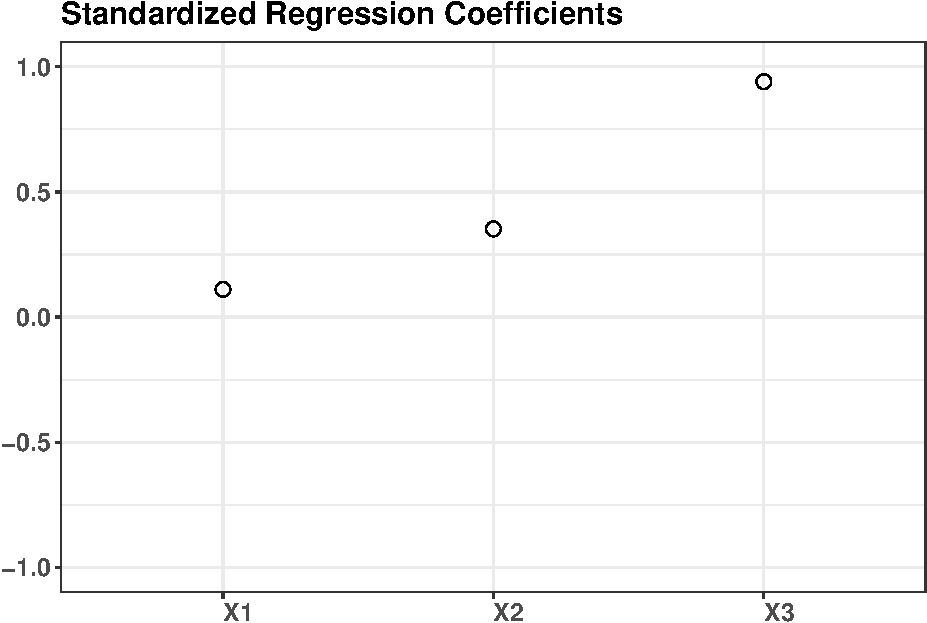
\includegraphics{topics_in_data_science_files/figure-latex/unnamed-chunk-2-1.pdf}

\begin{Shaded}
\begin{Highlighting}[]
\NormalTok{y }\OtherTok{\textless{}{-}} \FunctionTok{with}\NormalTok{(X, X1 }\SpecialCharTok{+}\NormalTok{ X2 }\SpecialCharTok{+}\NormalTok{ X3)}
\NormalTok{y }\OtherTok{\textless{}{-}}\NormalTok{ y }\SpecialCharTok{+} \FunctionTok{rnorm}\NormalTok{(}\FunctionTok{nrow}\NormalTok{(X),}\DecValTok{0}\NormalTok{,}\DecValTok{1}\SpecialCharTok{/}\DecValTok{2}\NormalTok{)}
\NormalTok{df}\OtherTok{\textless{}{-}} \FunctionTok{data.frame}\NormalTok{(}\FunctionTok{cbind}\NormalTok{(X,y))}

\NormalTok{Z }\OtherTok{\textless{}{-}} \FunctionTok{src}\NormalTok{(X, y, }\AttributeTok{rank =} \ConstantTok{FALSE}\NormalTok{, }\AttributeTok{logistic =} \ConstantTok{FALSE}\NormalTok{, }\AttributeTok{nboot =} \DecValTok{0}\NormalTok{, }\AttributeTok{conf =} \FloatTok{0.95}\NormalTok{)}

\FunctionTok{pander}\NormalTok{(Z}\SpecialCharTok{$}\NormalTok{SRC,}\AttributeTok{caption =} \StringTok{"Standardized Regression Coefficients "}\NormalTok{)}
\end{Highlighting}
\end{Shaded}

\begin{longtable}[]{@{}cc@{}}
\caption{Standardized Regression Coefficients}\tabularnewline
\toprule
\begin{minipage}[b]{0.12\columnwidth}\centering
~\strut
\end{minipage} & \begin{minipage}[b]{0.14\columnwidth}\centering
original\strut
\end{minipage}\tabularnewline
\midrule
\endfirsthead
\toprule
\begin{minipage}[b]{0.12\columnwidth}\centering
~\strut
\end{minipage} & \begin{minipage}[b]{0.14\columnwidth}\centering
original\strut
\end{minipage}\tabularnewline
\midrule
\endhead
\begin{minipage}[t]{0.12\columnwidth}\centering
\textbf{X1}\strut
\end{minipage} & \begin{minipage}[t]{0.14\columnwidth}\centering
0.08958\strut
\end{minipage}\tabularnewline
\begin{minipage}[t]{0.12\columnwidth}\centering
\textbf{X2}\strut
\end{minipage} & \begin{minipage}[t]{0.14\columnwidth}\centering
0.3392\strut
\end{minipage}\tabularnewline
\begin{minipage}[t]{0.12\columnwidth}\centering
\textbf{X3}\strut
\end{minipage} & \begin{minipage}[t]{0.14\columnwidth}\centering
0.9295\strut
\end{minipage}\tabularnewline
\bottomrule
\end{longtable}

\begin{Shaded}
\begin{Highlighting}[]
\FunctionTok{ggplot}\NormalTok{(Z, }\AttributeTok{ylim =} \FunctionTok{c}\NormalTok{(}\SpecialCharTok{{-}}\DecValTok{1}\NormalTok{,}\DecValTok{1}\NormalTok{))}\SpecialCharTok{+}\FunctionTok{ggtitle}\NormalTok{(}\StringTok{"Standardized Regression Coefficients"}\NormalTok{)}
\end{Highlighting}
\end{Shaded}

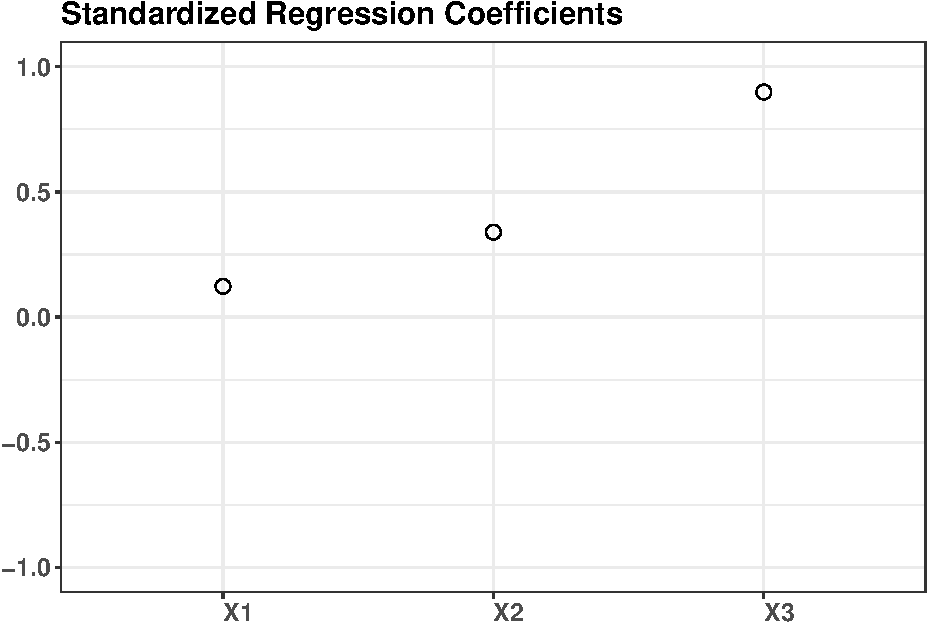
\includegraphics{topics_in_data_science_files/figure-latex/unnamed-chunk-3-1.pdf}

\begin{Shaded}
\begin{Highlighting}[]
\CommentTok{\#lm.fit = lm(y \textasciitilde{} X1+X2+X3,data = df)}
\CommentTok{\#summary(lm.fit)}
\CommentTok{\#attach(df)}
\CommentTok{\#plot(y, X1+X2+X3)}
\end{Highlighting}
\end{Shaded}

We see how the importance of X3 is ranked above X2 and likewise X2 is more important than X1. This is by design of the simulated data set. The standardized regression coefficients (beta coefficients) are calculated from that has been standardized, let's normalize and calculate the regression to see if indeed that is the case.

\begin{Shaded}
\begin{Highlighting}[]
\NormalTok{dfs}\OtherTok{\textless{}{-}} \FunctionTok{data.frame}\NormalTok{(}\FunctionTok{scale}\NormalTok{(df,}\AttributeTok{center =} \ConstantTok{TRUE}\NormalTok{,}\AttributeTok{scale =} \ConstantTok{TRUE}\NormalTok{))}
\NormalTok{lm.fit }\OtherTok{=} \FunctionTok{lm}\NormalTok{(y }\SpecialCharTok{\textasciitilde{}}\NormalTok{ X1}\SpecialCharTok{+}\NormalTok{X2}\SpecialCharTok{+}\NormalTok{X3,}\AttributeTok{data =}\NormalTok{ dfs)}
\FunctionTok{summary}\NormalTok{(lm.fit)}
\end{Highlighting}
\end{Shaded}

\begin{verbatim}
## 
## Call:
## lm(formula = y ~ X1 + X2 + X3, data = dfs)
## 
## Residuals:
##      Min       1Q   Median       3Q      Max 
## -0.60361 -0.09522 -0.00626  0.08943  0.40125 
## 
## Coefficients:
##              Estimate Std. Error t value Pr(>|t|)    
## (Intercept) 3.054e-16  1.769e-02   0.000        1    
## X1          8.958e-02  1.793e-02   4.998 2.61e-06 ***
## X2          3.392e-01  1.781e-02  19.047  < 2e-16 ***
## X3          9.295e-01  1.790e-02  51.942  < 2e-16 ***
## ---
## Signif. codes:  0 '***' 0.001 '**' 0.01 '*' 0.05 '.' 0.1 ' ' 1
## 
## Residual standard error: 0.1769 on 96 degrees of freedom
## Multiple R-squared:  0.9696, Adjusted R-squared:  0.9687 
## F-statistic:  1022 on 3 and 96 DF,  p-value: < 2.2e-16
\end{verbatim}

We see that the values are very close.

\hypertarget{partial-correlation-coefficients}{%
\section{Partial Correlation Coefficients}\label{partial-correlation-coefficients}}

\begin{Shaded}
\begin{Highlighting}[]
\NormalTok{x }\OtherTok{\textless{}{-}} \FunctionTok{pcc}\NormalTok{(X, y, }\AttributeTok{nboot =} \DecValTok{100}\NormalTok{)}
\FunctionTok{print}\NormalTok{(x)}
\end{Highlighting}
\end{Shaded}

\begin{verbatim}
## 
## Call:
## pcc(X = X, y = y, nboot = 100)
## 
## Partial Correlation Coefficients (PCC):
##     original          bias  std. error min. c.i. max. c.i.
## X1 0.4543671  0.0041092337 0.080517838 0.2860613 0.6075130
## X2 0.8892416 -0.0011730747 0.018469869 0.8569707 0.9281357
## X3 0.9826698 -0.0001722503 0.003255498 0.9766680 0.9903750
\end{verbatim}

\hypertarget{sobol-indices-for-deterministic-function-and-for-model}{%
\section{Sobol indices for deterministic function and for model}\label{sobol-indices-for-deterministic-function-and-for-model}}

\begin{Shaded}
\begin{Highlighting}[]
\NormalTok{y.fun }\OtherTok{\textless{}{-}} \ControlFlowTok{function}\NormalTok{(X) \{}
  
\NormalTok{  X1}\OtherTok{\textless{}{-}}\NormalTok{ X[,}\DecValTok{1}\NormalTok{]}
\NormalTok{  X2}\OtherTok{\textless{}{-}}\NormalTok{ X[,}\DecValTok{2}\NormalTok{]}
\NormalTok{  X3}\OtherTok{\textless{}{-}}\NormalTok{ X[,}\DecValTok{3}\NormalTok{]}
  
\NormalTok{  X1}\SpecialCharTok{+}\NormalTok{X2}\SpecialCharTok{+}\NormalTok{X3}
\NormalTok{\}}

\NormalTok{yhat.fun}\OtherTok{\textless{}{-}}\ControlFlowTok{function}\NormalTok{(X,lm)}
\NormalTok{\{}
\NormalTok{  X1}\OtherTok{\textless{}{-}}\NormalTok{ X[,}\DecValTok{1}\NormalTok{]}
\NormalTok{  X2}\OtherTok{\textless{}{-}}\NormalTok{ X[,}\DecValTok{2}\NormalTok{]}
\NormalTok{  X3}\OtherTok{\textless{}{-}}\NormalTok{ X[,}\DecValTok{3}\NormalTok{]}
  
\NormalTok{  yhat }\OtherTok{\textless{}{-}} \FunctionTok{predict}\NormalTok{(lm.fit,}\FunctionTok{data.frame}\NormalTok{(}\AttributeTok{X1=}\NormalTok{X1,}\AttributeTok{X2=}\NormalTok{X2,}\AttributeTok{X3=}\NormalTok{X3))}
  \FunctionTok{return}\NormalTok{(yhat)}
\NormalTok{\}}

\NormalTok{nboot }\OtherTok{=} \DecValTok{1000}

\NormalTok{x }\OtherTok{\textless{}{-}} \FunctionTok{sobol}\NormalTok{(}\AttributeTok{model =}\NormalTok{ y.fun, X[}\DecValTok{1}\SpecialCharTok{:}\DecValTok{50}\NormalTok{,], X[}\DecValTok{51}\SpecialCharTok{:}\DecValTok{100}\NormalTok{,], }\AttributeTok{order =} \DecValTok{3}\NormalTok{, }\AttributeTok{nboot =}\NormalTok{ nboot)}
\NormalTok{S.sobol }\OtherTok{\textless{}{-}}\NormalTok{ x}\SpecialCharTok{$}\NormalTok{S}
\FunctionTok{pander}\NormalTok{(S.sobol)}
\end{Highlighting}
\end{Shaded}

\begin{longtable}[]{@{}cccccc@{}}
\toprule
\begin{minipage}[b]{0.17\columnwidth}\centering
~\strut
\end{minipage} & \begin{minipage}[b]{0.12\columnwidth}\centering
original\strut
\end{minipage} & \begin{minipage}[b]{0.12\columnwidth}\centering
bias\strut
\end{minipage} & \begin{minipage}[b]{0.15\columnwidth}\centering
std. error\strut
\end{minipage} & \begin{minipage}[b]{0.14\columnwidth}\centering
min. c.i.\strut
\end{minipage} & \begin{minipage}[b]{0.14\columnwidth}\centering
max. c.i.\strut
\end{minipage}\tabularnewline
\midrule
\endhead
\begin{minipage}[t]{0.17\columnwidth}\centering
\textbf{X1}\strut
\end{minipage} & \begin{minipage}[t]{0.12\columnwidth}\centering
1.302\strut
\end{minipage} & \begin{minipage}[t]{0.12\columnwidth}\centering
0.04949\strut
\end{minipage} & \begin{minipage}[t]{0.15\columnwidth}\centering
0.8788\strut
\end{minipage} & \begin{minipage}[t]{0.14\columnwidth}\centering
-0.5695\strut
\end{minipage} & \begin{minipage}[t]{0.14\columnwidth}\centering
2.849\strut
\end{minipage}\tabularnewline
\begin{minipage}[t]{0.17\columnwidth}\centering
\textbf{X2}\strut
\end{minipage} & \begin{minipage}[t]{0.12\columnwidth}\centering
1.494\strut
\end{minipage} & \begin{minipage}[t]{0.12\columnwidth}\centering
0.04884\strut
\end{minipage} & \begin{minipage}[t]{0.15\columnwidth}\centering
0.8287\strut
\end{minipage} & \begin{minipage}[t]{0.14\columnwidth}\centering
-0.4242\strut
\end{minipage} & \begin{minipage}[t]{0.14\columnwidth}\centering
3.045\strut
\end{minipage}\tabularnewline
\begin{minipage}[t]{0.17\columnwidth}\centering
\textbf{X3}\strut
\end{minipage} & \begin{minipage}[t]{0.12\columnwidth}\centering
1.527\strut
\end{minipage} & \begin{minipage}[t]{0.12\columnwidth}\centering
0.03317\strut
\end{minipage} & \begin{minipage}[t]{0.15\columnwidth}\centering
0.3645\strut
\end{minipage} & \begin{minipage}[t]{0.14\columnwidth}\centering
0.76\strut
\end{minipage} & \begin{minipage}[t]{0.14\columnwidth}\centering
2.196\strut
\end{minipage}\tabularnewline
\begin{minipage}[t]{0.17\columnwidth}\centering
**X1*X2**\strut
\end{minipage} & \begin{minipage}[t]{0.12\columnwidth}\centering
-1.453\strut
\end{minipage} & \begin{minipage}[t]{0.12\columnwidth}\centering
-0.05783\strut
\end{minipage} & \begin{minipage}[t]{0.15\columnwidth}\centering
0.8793\strut
\end{minipage} & \begin{minipage}[t]{0.14\columnwidth}\centering
-2.996\strut
\end{minipage} & \begin{minipage}[t]{0.14\columnwidth}\centering
0.4286\strut
\end{minipage}\tabularnewline
\begin{minipage}[t]{0.17\columnwidth}\centering
**X1*X3**\strut
\end{minipage} & \begin{minipage}[t]{0.12\columnwidth}\centering
-1.453\strut
\end{minipage} & \begin{minipage}[t]{0.12\columnwidth}\centering
-0.05783\strut
\end{minipage} & \begin{minipage}[t]{0.15\columnwidth}\centering
0.8793\strut
\end{minipage} & \begin{minipage}[t]{0.14\columnwidth}\centering
-2.996\strut
\end{minipage} & \begin{minipage}[t]{0.14\columnwidth}\centering
0.4286\strut
\end{minipage}\tabularnewline
\begin{minipage}[t]{0.17\columnwidth}\centering
**X2*X3**\strut
\end{minipage} & \begin{minipage}[t]{0.12\columnwidth}\centering
-1.453\strut
\end{minipage} & \begin{minipage}[t]{0.12\columnwidth}\centering
-0.05783\strut
\end{minipage} & \begin{minipage}[t]{0.15\columnwidth}\centering
0.8793\strut
\end{minipage} & \begin{minipage}[t]{0.14\columnwidth}\centering
-2.996\strut
\end{minipage} & \begin{minipage}[t]{0.14\columnwidth}\centering
0.4286\strut
\end{minipage}\tabularnewline
\begin{minipage}[t]{0.17\columnwidth}\centering
\textbf{X1\emph{X2}X3}\strut
\end{minipage} & \begin{minipage}[t]{0.12\columnwidth}\centering
1.453\strut
\end{minipage} & \begin{minipage}[t]{0.12\columnwidth}\centering
0.05783\strut
\end{minipage} & \begin{minipage}[t]{0.15\columnwidth}\centering
0.8793\strut
\end{minipage} & \begin{minipage}[t]{0.14\columnwidth}\centering
-0.4286\strut
\end{minipage} & \begin{minipage}[t]{0.14\columnwidth}\centering
2.996\strut
\end{minipage}\tabularnewline
\bottomrule
\end{longtable}

\begin{Shaded}
\begin{Highlighting}[]
\CommentTok{\#yhat.fun(data.frame(X1=1,X2=2,X3=3),lm.fit)}

\NormalTok{x }\OtherTok{\textless{}{-}} \FunctionTok{sobol}\NormalTok{(}\AttributeTok{model =}\NormalTok{ yhat.fun,X[}\DecValTok{1}\SpecialCharTok{:}\DecValTok{50}\NormalTok{,], X[}\DecValTok{51}\SpecialCharTok{:}\DecValTok{100}\NormalTok{,], }\AttributeTok{order =} \DecValTok{3}\NormalTok{, }\AttributeTok{nboot =}\NormalTok{ nboot)}
\NormalTok{S.sobol }\OtherTok{\textless{}{-}}\NormalTok{ x}\SpecialCharTok{$}\NormalTok{S}
\FunctionTok{pander}\NormalTok{(S.sobol)}
\end{Highlighting}
\end{Shaded}

\begin{longtable}[]{@{}cccccc@{}}
\toprule
\begin{minipage}[b]{0.17\columnwidth}\centering
~\strut
\end{minipage} & \begin{minipage}[b]{0.12\columnwidth}\centering
original\strut
\end{minipage} & \begin{minipage}[b]{0.12\columnwidth}\centering
bias\strut
\end{minipage} & \begin{minipage}[b]{0.15\columnwidth}\centering
std. error\strut
\end{minipage} & \begin{minipage}[b]{0.14\columnwidth}\centering
min. c.i.\strut
\end{minipage} & \begin{minipage}[b]{0.14\columnwidth}\centering
max. c.i.\strut
\end{minipage}\tabularnewline
\midrule
\endhead
\begin{minipage}[t]{0.17\columnwidth}\centering
\textbf{X1}\strut
\end{minipage} & \begin{minipage}[t]{0.12\columnwidth}\centering
1.064\strut
\end{minipage} & \begin{minipage}[t]{0.12\columnwidth}\centering
0.04465\strut
\end{minipage} & \begin{minipage}[t]{0.15\columnwidth}\centering
0.7367\strut
\end{minipage} & \begin{minipage}[t]{0.14\columnwidth}\centering
-0.476\strut
\end{minipage} & \begin{minipage}[t]{0.14\columnwidth}\centering
2.395\strut
\end{minipage}\tabularnewline
\begin{minipage}[t]{0.17\columnwidth}\centering
\textbf{X2}\strut
\end{minipage} & \begin{minipage}[t]{0.12\columnwidth}\centering
1.064\strut
\end{minipage} & \begin{minipage}[t]{0.12\columnwidth}\centering
0.04445\strut
\end{minipage} & \begin{minipage}[t]{0.15\columnwidth}\centering
0.7332\strut
\end{minipage} & \begin{minipage}[t]{0.14\columnwidth}\centering
-0.4372\strut
\end{minipage} & \begin{minipage}[t]{0.14\columnwidth}\centering
2.384\strut
\end{minipage}\tabularnewline
\begin{minipage}[t]{0.17\columnwidth}\centering
\textbf{X3}\strut
\end{minipage} & \begin{minipage}[t]{0.12\columnwidth}\centering
1.324\strut
\end{minipage} & \begin{minipage}[t]{0.12\columnwidth}\centering
0.01343\strut
\end{minipage} & \begin{minipage}[t]{0.15\columnwidth}\centering
0.1234\strut
\end{minipage} & \begin{minipage}[t]{0.14\columnwidth}\centering
1.043\strut
\end{minipage} & \begin{minipage}[t]{0.14\columnwidth}\centering
1.533\strut
\end{minipage}\tabularnewline
\begin{minipage}[t]{0.17\columnwidth}\centering
**X1*X2**\strut
\end{minipage} & \begin{minipage}[t]{0.12\columnwidth}\centering
-1.078\strut
\end{minipage} & \begin{minipage}[t]{0.12\columnwidth}\centering
-0.04514\strut
\end{minipage} & \begin{minipage}[t]{0.15\columnwidth}\centering
0.7354\strut
\end{minipage} & \begin{minipage}[t]{0.14\columnwidth}\centering
-2.409\strut
\end{minipage} & \begin{minipage}[t]{0.14\columnwidth}\centering
0.4652\strut
\end{minipage}\tabularnewline
\begin{minipage}[t]{0.17\columnwidth}\centering
**X1*X3**\strut
\end{minipage} & \begin{minipage}[t]{0.12\columnwidth}\centering
-1.078\strut
\end{minipage} & \begin{minipage}[t]{0.12\columnwidth}\centering
-0.04514\strut
\end{minipage} & \begin{minipage}[t]{0.15\columnwidth}\centering
0.7354\strut
\end{minipage} & \begin{minipage}[t]{0.14\columnwidth}\centering
-2.409\strut
\end{minipage} & \begin{minipage}[t]{0.14\columnwidth}\centering
0.4652\strut
\end{minipage}\tabularnewline
\begin{minipage}[t]{0.17\columnwidth}\centering
**X2*X3**\strut
\end{minipage} & \begin{minipage}[t]{0.12\columnwidth}\centering
-1.078\strut
\end{minipage} & \begin{minipage}[t]{0.12\columnwidth}\centering
-0.04514\strut
\end{minipage} & \begin{minipage}[t]{0.15\columnwidth}\centering
0.7354\strut
\end{minipage} & \begin{minipage}[t]{0.14\columnwidth}\centering
-2.409\strut
\end{minipage} & \begin{minipage}[t]{0.14\columnwidth}\centering
0.4652\strut
\end{minipage}\tabularnewline
\begin{minipage}[t]{0.17\columnwidth}\centering
\textbf{X1\emph{X2}X3}\strut
\end{minipage} & \begin{minipage}[t]{0.12\columnwidth}\centering
1.078\strut
\end{minipage} & \begin{minipage}[t]{0.12\columnwidth}\centering
0.04514\strut
\end{minipage} & \begin{minipage}[t]{0.15\columnwidth}\centering
0.7354\strut
\end{minipage} & \begin{minipage}[t]{0.14\columnwidth}\centering
-0.4652\strut
\end{minipage} & \begin{minipage}[t]{0.14\columnwidth}\centering
2.409\strut
\end{minipage}\tabularnewline
\bottomrule
\end{longtable}

\hypertarget{random-effects-and-mixed-models}{%
\chapter{Random Effects and Mixed Models}\label{random-effects-and-mixed-models}}

\hypertarget{crossed-versus-nested-random-effects.}{%
\section{Crossed versus nested random effects.}\label{crossed-versus-nested-random-effects.}}

How do they differ and how are they specified correctly in lme4 and in JAGS / Stan?

\hypertarget{very-large-number-of-res}{%
\section{Very Large Number of RE's}\label{very-large-number-of-res}}

\url{https://arxiv.org/abs/1610.08088}

\hypertarget{propensity-score-matching}{%
\chapter{Propensity Score Matching}\label{propensity-score-matching}}

\hypertarget{caliper}{%
\section{Caliper}\label{caliper}}

Putting constraints on matching can reduce bias \citep{10.1093/aje/kwt212}.

\emph{Matching on the propensity score is widely used to estimate the effect of an exposure in observational studies. However, the quality of the matches can be affected by decisions made during the matching process, particularly the order in which subjects are selected for matching and the maximum permitted difference between matched subjects (the ``caliper''). This study used simulations to explore the effects of these decisions on both the imbalance of covariates and the closeness of matching, while allowing the numbers of potential matches and strengths of association between the confounding variable and the exposure to vary. It was found that, without a caliper, substantial bias was possible, particularly with a relatively small reservoir of potential matches and strong confounder-exposure association. Use of the recommended caliper reduced the bias considerably, but bias remained if subjects were selected by increasing or decreasing propensity score. A tighter caliper led to greatly reduced bias and closer matches, although some subjects could not be matched. This study suggests that a narrow caliper can improve the performance of propensity score matching. In situations where it is impossible to find appropriate matches for all exposed subjects, it is better to select subjects in order of the best available matches, rather than increasing or decreasing the propensity score.}

\hypertarget{introduction-to-normalizing-flows}{%
\chapter{Introduction to Normalizing Flows}\label{introduction-to-normalizing-flows}}

\hypertarget{variational-inference-with-nf}{%
\section{Variational Inference With NF}\label{variational-inference-with-nf}}

\emph{Variational inference now lies at the core of large-scale topic models of text (Hoffman et al., 2013), provides the state-of-the-art in semi-supervised classification (Kingma et al., 2014), drives the models that currently produce the most realistic generative models of images (Gregor et al., 2014; Rezende et al., 2014), and are a default Proceedings of the 32 nd International Conference on Machine Learning, Lille, France, 2015. JMLR: W\&CP volume 37. Copyright 2015 by the author(s). tool for the understanding of many physical and chemical systems. Despite these successes and ongoing advances, there are a number of disadvantages of variational methods that limit their power and hamper their wider adoption as a default method for statistical inference. It is one of these limitations, the choice of posterior approximation, that we address in this paper}

{[}\url{http://proceedings.mlr.press/v37/rezende15.pdf}{]}

\emph{Generative modeling loosely refers to building a model of data, for instance p(image), that we can sample from. This is in contrast to discriminative modeling, such as regression or classification, which tries to estimate conditional distributions such as p(class \textbar{} image).}

\hypertarget{section}{%
\section{}\label{section}}

  \bibliography{packages.bib,book.bib}

\end{document}
